\documentclass[11pt,letterpaper]{article}
\usepackage[margin=.88in]{geometry}
\usepackage{amsmath,amssymb,amsthm,mathtools,booktabs,array,tabularx,tikz,microtype,enumitem,hyperref,fancyhdr,lastpage}
\usetikzlibrary{arrows.meta,positioning}
\hypersetup{hidelinks,pdftitle={The Price of Knowing How to Improve},pdfauthor={Research direction: Brian Tenneson; mathematical drafting: ChatGPT}}
\pagestyle{fancy}\fancyhf{}\lhead{\small SCDF research extension 001v2}\rhead{\small Certified awareness and control}\cfoot{\thepage\ / \pageref{LastPage}}
\setlength{\headheight}{14pt}\setlength{\parskip}{.45em}\setlength{\parindent}{0pt}
\newtheorem{theorem}{Theorem}[section]\newtheorem{proposition}[theorem]{Proposition}\newtheorem{corollary}[theorem]{Corollary}\newtheorem{definition}[theorem]{Definition}
\newcommand{\E}{\mathbb E}\newcommand{\R}{\mathbb R}\newcommand{\N}{\mathbb N}\newcommand{\ind}{\mathbf 1}
\title{\textbf{The Price of Knowing How to Improve}\\[.5em]\large Certified Coalition Awareness, Paper-Benchmark Decisions, and Sovereign Clock Revision in SCDF}
\author{Research Director: Brian Tenneson\\ Mathematical development: Picard and DATA MIND (conversational research roles)\\ Internal adversarial review: Atlas (conversational research role)}
\date{November 25, 2026 \quad Research extension 001v2 (Atlas re-audit)}
\begin{document}
\maketitle
\begin{abstract}
A federation can know more about itself without becoming a better theorem prover. We make the missing implication precise in a finite, verifier-gated architecture-selection problem. Certified receipts induce partitions of hidden operational states; exact and interval-valued decision costs give paper certificates for the value of refinement. A finite decision tree characterizes optimal paid receipt acquisition. For every coalition size $n\ge2$, a parity-composition witness has zero gross decision value for every proper coalition, yet a strictly positive fully charged advantage for the whole coalition under an exact threshold. The construction separates mathematical settlement from meta-evidence and rules out greedy single-receipt acquisition as a general optimal policy. A second extension of the countably fair dyadic clock shows how an independently admitted, identity-preserving clock gift can promote an identified worker while retaining recurrent service for every worker. Its exact deadline and cost formulas give a restricted awareness-dependent sovereign separation. These are conditional mathematical results and finite model witnesses, not an assertion of universal gift admissibility, empirical ATP acceleration, or an independently executing federation.
\end{abstract}
\setcounter{tocdepth}{1}
\tableofcontents
\clearpage
\section{The three sources and the new question}
The supplied \emph{Formalized Awareness of AMLD Federations and Board-Players}, v0.3 (A) separates object proofs, accessible meta-warrants, individual and federation awareness, and coalition-dependent reflective surplus. Its Definition 6.2 and Proposition 6.4 give a three-source Horn dependency witness. Section 7 explicitly refuses to infer operational advantage from reflective surplus; Propositions 7.2 and Theorem 7.3 give no-free-reflection barriers when the comparator can imitate the policy, including costs. Its Theorem 5.3 gives a computable countably recurrently fair clock \cite{aware}.

\emph{Before the Clock Starts}, audited 001v2 (B), freezes the workload, comparator, information, permissions, and cost metric (Definition 1.1), separates paper proofs from modeled and physical timing (Sections 2--4), and gives cost-dominating imitation and certified interval closure (Theorems 7.1 and 8.1). Its Section 9 charges the acquisition of better benchmarks themselves \cite{bench}.

\emph{Who Checks the Federation?}, 7.10v2 (C), supplies the separate Board/BANK boundary, typed dependence records with open obligations, source-scoped proof composition, and matched comparison discipline. In particular its Proposition 19.1 allows reflective information to select methods but not alter theoremhood, while Theorem 19.2 compares certified lower bounds with actual successful paths. Its v2 supplement repairs the placement of conditional D reports in the theorem BANK \cite{checks}.

SCDF 014v2 (S), its sovereign development (identified by the heading ``SCDF: the sovereign extension of CDF-C''), permits selected changes in schedule, generator interface or active permissions through parent-bound externally admitted gifts. The immutable external envelope includes the object checker, revision checker, identity, accounting and consistency obligations \cite{scdf}. We use that restricted mathematical contract, not a claim of an installed machine.

\begin{center}
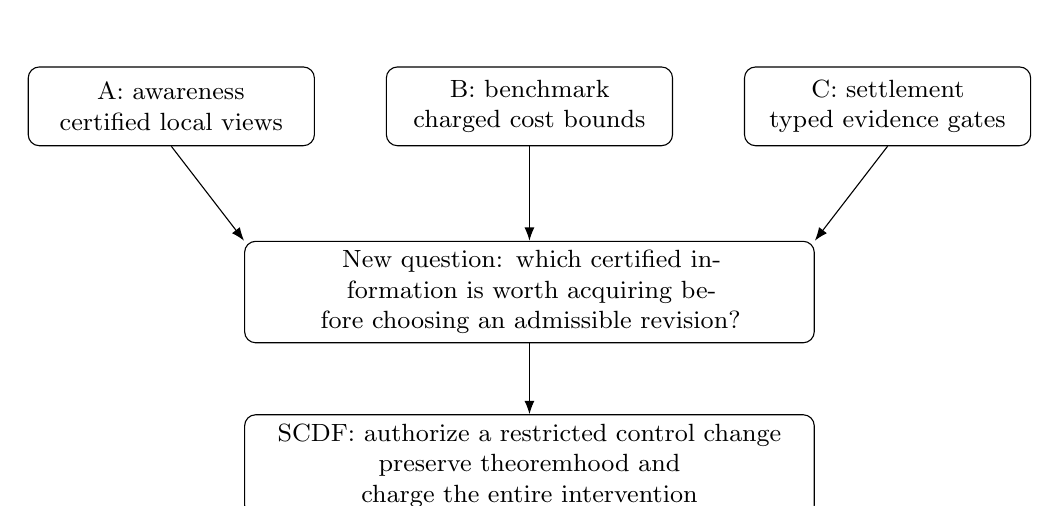
\begin{tikzpicture}[node distance=9mm, every node/.style={font=\small}, b/.style={draw,rounded corners,align=center,text width=3.4cm,minimum height=1cm}, >=Latex]
\node[b] (a) {A: awareness\\ certified local views};
\node[b,right=of a] (b) {B: benchmark\\ charged cost bounds};
\node[b,right=of b] (c) {C: settlement\\ typed evidence gates};
\node[b,below=12mm of b,text width=7cm] (d) {New question: which certified information is worth acquiring before choosing an admissible revision?};
\node[b,below=of d,text width=7cm] (e) {SCDF: authorize a restricted control change\\ preserve theoremhood and charge the entire intervention};
\draw[->] (a.south) -- (d.north west);\draw[->] (b) -- (d);\draw[->] (c.south) -- (d.north east);\draw[->] (d) -- (e);
\end{tikzpicture}
\end{center}
\textbf{Deductive target.} Extend structural coalition dependency to an exact decision-value statement, and connect the result to an admissible schedule change. This is an extension of the supplied statements, not a claim of priority over decision theory, information economics or scheduling literature. All new proofs are collected in Appendix A.

\section{A frozen reflective decision contract}
\begin{definition}[Receipt decision problem]\label{def:contract}
Fix a finite nonempty hidden operational state space $\Omega$, a full-support probability distribution $\mu$ when expected costs are used, a finite nonempty set $A$ of authorized terminal policies, and a nonnegative finite cost table $c(\omega,a)$. A terminal policy includes its required checks, failure recovery, and final settlement; every listed policy terminates successfully on every state. The object calculus, hypotheses, target, proof checker $V$, meta-checker $W$, sovereignty envelope and initial state distribution are fixed. The hidden state describes operational facts, not a secret change of mathematical truth. An action unavailable on some state can be modeled only by an explicitly authorized safe rejection/fallback policy with its complete cost, not by executing an illegal transition.

A finite indexed receipt family $Q$ consists of functions $f_i:\Omega\to O_i$ with finite ranges, and fixed acquisition costs $k_i\ge0$. Acquisition includes observation, authentication, translation, checking, delivery and storage. In this idealized contract each requested receipt succeeds, is accepted for the current epoch, is accessible to the decision maker, and reveals only its declared value. Any failed or stale receipt must be handled separately in an enlarged state model. No other observations are available before selecting a terminal policy. All policies in $A$ are available after any allowed receipt transcript (possibly with the declared rejection/fallback semantics). Within the unrestricted receipt problem every unused receipt is available at each query step. The external gate can see the source state needed for checking, but may not leak it outside the declared receipt interface, including through acceptance decisions, preparation costs, timing, or authorization responses. All randomness used by the controller is independent of the hidden state. Costs are fixed scalar charges in one metric; policy-tree design or proof of optimality is either supplied as common starting information or separately charged. The table includes all costs of executing a selected terminal policy but not the separately itemized receipt or gift charges.
\end{definition}
A subset $J\subseteq Q$ yields a partition $\mathcal P_J$ into nonempty fibers of the joint observation $f_J$. A decision rule selects a policy constant on each cell $E$ of that partition. In the expected-cost setting define
\[
 R(J)=\sum_{E\in\mathcal P_J}\mu(E)\min_{a\in A}\E[c(\omega,a)\mid E],\qquad
 g(J)=R(\varnothing)-R(J).
\]
$g$ is gross decision value, not the number of newly banked theorems. The acquisition cost of a fixed coalition is $k(J)=\sum_{i\in J}k_i$. For a deterministic guarantee define
\[
 D(J)=\max_{E\in\mathcal P_J}\min_{a\in A}\max_{\omega\in E}c(\omega,a).
\]
$D$ is worst-case complete cost for deterministic terminal policies. Randomized worst-case expected cost is a different metric. Expected-cost formulas allow independent randomized choices but deterministic policies suffice because the objective is linear in their action probabilities.

\begin{theorem}[Refinement and exact price of a fixed coalition]\label{thm:partition}
If $J\subseteq J'$, then $R(J')\le R(J)$ and $D(J')\le D(J)$. Under the fixed-coalition contract the optimal expected cost with $J$ is exactly $R(J)+k(J)$; the optimal deterministic worst-case cost is $D(J)+k(J)$. The coalition yields strict expected improvement over the receipt-blind optimum iff $g(J)>k(J)$. If a gift enabling the acquisition costs a further fixed $K\ge0$, replace $k(J)$ by $k(J)+K$.
\end{theorem}
A strict information refinement can leave both decision optima unchanged. Conversely an information refinement with large gross value may fail after paying for it. This replaces the qualitative gap in A, Section 7, with an exact criterion under a finite contract.

\begin{theorem}[Interval certificate for a decision improvement]\label{thm:interval}
Suppose the common cost table is bounded by sound compatible entrywise certificates $\ell(\omega,a)\le c(\omega,a)\le u(\omega,a)$, all finite. Define $R_\ell,R_u,D_\ell,D_u$ by replacing $c$ with the indicated endpoint table. Then
\[
 R_\ell(J)\le R(J)\le R_u(J),\qquad D_\ell(J)\le D(J)\le D_u(J).
\]
In particular $K+k(J)+R_u(J)<R_\ell(J_0)+k(J_0)$ certifies strict expected improvement over \emph{every} fixed-coalition-$J_0$ policy; the same inequality with $D$ proves strict separation in optimal deterministic worst-case cost. All charges must refer to the same metric and workload, with the two arms' permission differences explicitly declared. The displayed strict test assumes that the stated coalition choices are authorized in their respective arms and their acquisition and gift charges are exact; otherwise use an upper bound on the proposed arm's charges and a lower bound on the comparator's charges. For a comparator allowed to select among multiple coalitions, use a lower bound for the optimum over all its legal choices, not just one convenient coalition.
\end{theorem}
The bounds can be acquired by B's paper-benchmark inequalities. The act of tightening an interval is not itself a reduction of execution cost; the theorem tells us when those bounds justify a decision. Any additional charge to generate the bounds must appear in $K$ or another explicitly charged category, not vanish into the word ``certified.''

\section{The cost of discovering which receipt to read}
A fixed coalition is not always the best acquisition policy. The controller may decide which receipt to acquire next from information already accepted, without reading hidden state directly. Let $E\subseteq\Omega$ be a nonempty current fiber and $U\subseteq Q$ the unused receipt indices. In this section all unused receipts may be requested and the terminal action set is unchanged. Previously spent costs are sunk, and unused indices and the current fiber determine every remaining legal choice and charge. A receipt query splits $E$ into nonempty sets $E_{i,z}=\{\omega\in E:f_i(\omega)=z\}$. For a deterministic worst-case decision tree replace conditional probabilities by maximum over possible answers. Set
\[
 r(E)=\min_a\E[c(\omega,a)\mid E],\qquad d(E)=\min_a\max_{\omega\in E}c(\omega,a).
\]
\begin{theorem}[Exact adaptive acquisition frontier]\label{thm:bellman}
The minimum remaining expected total cost $F(E,U)$ of any legal acquisition tree is given by
\begin{align*}
 F(E,\varnothing)&=r(E),\\
 F(E,U)&=\min\left\{r(E),\min_{i\in U}\left[k_i+\sum_{z}\frac{\mu(E_{i,z})}{\mu(E)}F(E_{i,z},U\setminus\{i\})\right]\right\}.
\end{align*}
The sum is over nonempty fibers. The optimal deterministic worst-case remaining cost $G(E,U)$ satisfies the same recursion with $r$ replaced by $d$ and the weighted sum replaced by $\max_z$. Each optimum is attained by a finite legal tree. If a tree itself requires an additional design, verification or installation cost, the comparison must charge that cost separately. This is a finite mathematical optimizer, not a free or universally efficient implementation.
\end{theorem}
\textbf{A hard budget.} The worst-case recursion gives an exact feasibility test for a fixed available budget $B$: a deterministic tree settling on every hidden state exists iff $G(\Omega,Q)\le B$. If a gift is optional with upfront cost $K$, test $K+G(\Omega,Q)\le B$ for the gifted arm; the overall feasibility test is the disjunction with feasibility in the ungifted arm under its actual access restrictions. If permissions depend on query history, augment the state and minimize only over currently legal requests. For a cardinality cap, one can instead stop recursion once the cap is reached. The unrestricted recursion alone does not compute the value of an arbitrary stateful gate. Unlike minimizing average loss, this test prohibits a single branch from overrunning the budget. A more general expected objective under a hard cap requires a remaining-budget coordinate and infeasible branches excluded; no such cap is silently assumed in $F$.

\section{A quantitative Gestalt theorem}
A's three-source witness establishes that a proposition can require a whole coalition for its derivation. Here the whole coalition is indispensable to attaining the better decision optimum, even though every member's observation is individually true and checkable by the stipulated meta-checker. The result concerns the full parity value, not the inability of a proper coalition to derive any information at all.

\subsection{An explicit finite operational model}
Fix $n\ge2$. Let $\Omega=\{0,1\}^n$ with the uniform distribution. Agent $i$ holds a local, frozen orientation bit $x_i$. These bits describe the encodings of a chain of binary handoff interfaces: the $i$th interface applies $y\mapsto y\oplus x_i$. The composition is $y\mapsto y\oplus p(x)$, where $p(x)=x_1\oplus\cdots\oplus x_n$. A proposed fast route chooses a compensating orientation $b\in\{0,1\}$; its interface is compatible exactly if $b=p(x)$. Each receipt is a tagged assertion of the current orientation at its own interface. In the finite model the meta-checker compares the assertion to the exact frozen local state, checks source, epoch and authorization, and accepts a composition claim only with the complete list of admitted premises and a checked XOR calculation. For a common typed Boolean meta-theory of the orientation variables, every proper set of bit receipts has two models with opposite parity; the complete set determines the parity. This supplies a minimal-coalition dependence witness for the operational proposition $p(x)=b$ relative to the frozen initial views. Derivability alone is not a receipt; a federation-level claim still requires its own accepted scoped witness and access. The fixed receipt costs and gift cost include any composition check and delivery needed for the declared model (or an explicit zero incremental charge if included in another cost category). This is a sound table/replay model, not a deployed authentication system.

Take a fixed object theory $H=\{s,s\to t\}$ with a sound checker of modus ponens. The target is $t$ in all worlds. There is a slow authorized proof-delivery route $a_*$, costing $h>0$ including checking. Fast-route proposal $a_b$ costs $l$ on a match, where $0\le l<h$; the gate checks compatibility before transfer and the final object certificate is the same checked derivation of $t$. On mismatch the proposed transfer is rejected, the attempt is charged $w-h\ge0$, and the unchanged slow route executes, total $w$. The contract permits at most one fast-route attempt, no probing, free orientation test, direct unauthorized certificate write, or other legal route. The costs are stipulated full charges of this finite model, not time measurements. Role-local observations are held behind the authorization interface; a controller cannot read arbitrary local state merely because it schedules that role. The fallback is mandatory on mismatch. All cost information and the distribution are public; only $x$ is hidden.
\[
 c(x,a_*)=h,\qquad c(x,a_b)=\begin{cases}l&b=p(x),\\ w&b\ne p(x).\end{cases}
\]
Assume $w\ge2h-l$. Thus even a blind randomized guess cannot beat the slow route in expectation. In the constructive witness, a single optional permission gift is admissible for every $x$ and enables the sovereign to request and pool all $n$ receipts, preserving the same object verifier, proof theory and available terminal policies. Its admission is independent of the hidden parity and has the same cost $K$ in every state. The choice to grant or decline is made before the first receipt query; the decision maker has no extra input through the gift gate. This is a proposed restricted SCDF-native permission transition, not a general theorem of GBG+S gift admissibility. The comparator may read adaptively at most a proper subset along every path, and has no other source of orientation information. This is an explicitly restricted information-access contract; a singleton granted all identical rights is not excluded from the gifted performance.

\begin{theorem}[All-or-nothing decision value]\label{thm:parity}
For every proper coalition $J\subsetneq Q$, $R(J)=D(J)=h$; for the full coalition, $R(Q)=D(Q)=l$. The same baseline optimum $h$ holds even for adaptive queries that never complete the coalition, for expected cost, deterministic worst-case cost, and worst-case expected cost with independent randomization. Here worst-case expected cost means $\max_x\mathbb E_{\mathrm{seed}}[C(x,\mathrm{seed})]$, and $h$ is attained by choosing no queries and the slow route. Hence
\[
 g(J)=\begin{cases}0&J\subsetneq Q,\\h-l&J=Q.\end{cases}
\]
With nonnegative query costs and a fixed upfront permission-gift cost $K$, the optimum of the architecture that may decline the gift or acquire any coalition is, both in expected cost and deterministic worst-case cost,
\[
 \boxed{\min\{h,\ l+K+\textstyle\sum_{i=1}^n k_i\}.}
\]
Full-coalition acquisition is strictly advantageous iff $K+\sum_i k_i<h-l$. This holds against the best policy in the stated restricted baseline, not merely a chosen blind policy. Both architectures settle the same object theorem; the gain is a charged control advantage.
\end{theorem}
\begin{corollary}[A greedy obstruction]\label{cor:greedy}
If $k_i>0$ for all $i$ and $K+\sum_i k_i<h-l$, a policy that acquires only a receipt having strictly positive immediate net decision value stops at the empty coalition, although full acquisition is strictly beneficial. The gross set function $g$ is not submodular: all proper coalitions have value zero and adding the last receipt has marginal value $h-l>0$.
\end{corollary}
The obstruction applies to this specified myopic rule, not every heuristic called greedy. It suggests that a revision generator should sometimes propose a jointly justified bundle rather than insist on individually profitable first moves. The independent gate must still validate every member and its cumulative context.

\subsection{Three-source numerical witness}
Take $n=3$, $h=8$, $l=2$, $w=14$, $k_i=1$, $K=1$. The stipulated costs satisfy $w=2h-l$. Reading all three and committing the gift costs $1+3+2=6$; the best receipt-restricted baseline costs $8$. Every proper coalition has zero gross decision value. Acquisition without completing the coalition worsens cost when it incurs positive charges.
\begin{center}
\begin{tabular}{lrrr}
\toprule
Information & Best terminal expected cost & Receipt charges & Total before gift \\
\midrule
None & 8 & 0 & 8\\
Any one & 8 & 1 & 9\\
Any pair & 8 & 2 & 10\\
All three & 2 & 3 & 5\\
\bottomrule
\end{tabular}
\end{center}
\begin{center}
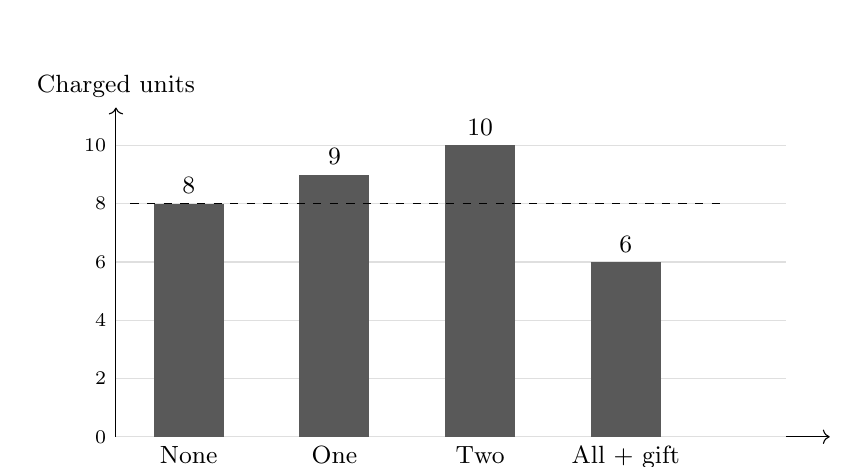
\begin{tikzpicture}[x=1.85cm,y=.37cm]
\draw[->] (-.5,0)--(4.4,0);\draw[->] (-.5,0)--(-.5,11.3) node[above,font=\small]{Charged units};
\foreach \y in {0,2,4,6,8,10}{\draw[gray!25] (-.5,\y)--(4.1,\y);\node[left,font=\scriptsize] at (-.5,\y){\y};}
\foreach \x/\y/\lab in {0/8/None,1/9/One,2/10/Two,3/6/All + gift}{\fill[black!65] (\x-.24,0) rectangle (\x+.24,\y);\node[above,font=\small] at (\x,\y){\y};\node[below,font=\small] at (\x,0){\lab};}
\draw[dashed] (-.4,8)--(3.7,8);\end{tikzpicture}
\end{center}
\textit{Caption.} Fully charged fixed-policy comparison; partial arms have no gift cost (a favorable lower cost for the comparator), and the all-three arm includes it. Cost units are synthetic.

\section{Awareness-dependent fair clock promotion}
The first witness concerned the cost of choosing a compatible policy. We now extend the countably fair clock from A, Theorem 5.3, and the clock-rewrite witness from SCDF 014v2. The goal is to change access to scarce service slots without erasing any worker's infinite-horizon service guarantee.

\begin{definition}[Interleaved dyadic service contract]\label{def:clock}
Let $S$ be one sovereign office and let $a_i$, $i\in\N=\{0,1,\ldots\}$, be an effectively indexed set of worker identities. Each nonnegative even tick belongs to $S$, and at odd tick $2s+1$ the baseline serves $a_{v_2(s+1)}$. A finite permutation $\pi$ of the worker indices (identity off finite support) may be installed only at the initial tick 0 by a B14-style clock gift, with a positive parent-bound external authorization and preservation witness. The resulting schedule is
\[
 \chi_\pi(2s)=S,\qquad \chi_\pi(2s+1)=a_{\pi(v_2(s+1))}.
\]
The original schedule is used at the commit boundary. No worker is created or destroyed, no credit is minted, and the unique sovereign and checker are unchanged. A known total effective step selector, including permitted charged no-ops, is required; the schedule alone does not imply discovery. An infinite run is a mathematical service model, not a finite-budget deployment. For a finite trial only its finite prefix is executed; an external contract may use effective on-demand worker state, rather than preinstantiating infinitely many processes.
\end{definition}
\begin{theorem}[Exact recurrence-preserving promotion]\label{thm:clock}
Every such schedule is computable and recurrently fair for $S$ and every worker. The gap for $a_j$ is exactly $2^{\pi^{-1}(j)+2}$ ticks. Suppose a fixed designated worker $a_j$ ($j\ge1$) needs exactly $m\ge1$ of its own committed services to submit and settle a target, with checking charged within the service contract, and no other worker can settle it or interfere. The baseline completion tick-count (including tick 0) and the count after the transposition $(0\ j)$ are
\[
 d_j(m)=2^{j+1}(2m-1),\qquad d_g(m)=2(2m-1).
\]
Thus if every tick costs one common unit, equal other costs cancel and the gift incurs total incremental non-tick charge $K$, it strictly lowers charged cost exactly when
\[
 K<(2^{j+1}-2)(2m-1).
\]
The witness is for a specified service model, with acquisition and gift preparation completed before or within tick 0 and fully charged separately, with a valid receipt for the exact current parent. These activities do not consume additional service slots in this trial. The common object checking cost is already included in the declared per-service charge or the equal other costs; it is not counted twice. If preparation consumes extra service ticks, the formula must include them. No uniform common finite recurrence gap is created for countably many workers.
\end{theorem}

\begin{corollary}[The hidden-worker separation]\label{cor:hidden}
Consider the same uniform $n$-bit states and authenticated receipt interface of Section 4, now with the designated worker $j=1+p(x)$. The only permitted initial rewrite is one of the two transpositions $(0\ 1)$ or $(0\ 2)$; declining is also allowed. Both transpositions satisfy the same structural admission contract for every hidden state, and admission, receipt access, budget and preparation supply no further information about $j$. In particular the gate does not test whether the proposed transposition promotes the target-producing worker. The designated worker's proof progress and service telemetry are not available until after the irrevocable initial choice; no later rewrite is legal. The precommit receipts describe the frozen workload/worker assignment, which is invariant under the permutation, and are valid for that parent. They need not be reinterpreted as claims about the postcommit clock. The ordinary proof interface is frozen, and the target requires exactly $m\ge2$ services from the designated worker. At deadline $d=2(2m-1)$, a controller with all receipts and an admitted matching gift guarantees settlement on every state. A controller with only a proper subset along every observation path cannot guarantee settlement, even if granted the same two rewrite choices. With a uniform hidden state any such possibly randomized controller succeeds with probability at most $1/2$ by that deadline. This upper bound is attained by choosing either fixed transposition without queries, when its admitted cost fits the budget. The comparator cannot use an authorization failure, a trial rewrite, a target-specific hint or a second clock decision as a free parity query. The no-rewrite baseline fails on every state.
\end{corollary}
This deadline is counted from the clock epoch, not from the beginning of receipt acquisition. The comparison includes identical service deadlines and a sufficient common charged budget for both arms, including all receipt and gift expenses. To compare total elapsed physical latency one needs a separate duration model, just as B requires. For $m=2$, the baseline completion counts are 12 or 24, and a matching promotion completes in six service ticks. Neither the awareness result nor the fair-clock result alone implies the combined separation.

\section{Evidence gates and limits of the extension}
\begin{proposition}[A typed preservation and imitation boundary]\label{prop:boundary}
Assume the same sound object checker $V$, immutable object hypotheses, initially sound admitted object records, and finite well-founded scoped proof dependencies for every state and both arms. All ordinary transitions that can modify the object store obey the object-commit gate; no alternate writer is permitted. Let meta-receipts and revision evidence enter a separate typed store, with no import rule turning them into object premises. Admit an action changing active receipt permission or clock only after a sound external gate checks its exact parent, authorization, cumulative consistency and operational preservation; unknown or rejected evidence never activates the change. Then every accepted object theorem in a finite mixed history is an object consequence of the original hypotheses, regardless of the receipt-selection policy. Under these assumptions the examples do not prove intrinsic non-singleton superiority: any comparator admitting a causal, legal policy translation that preserves the observation interface, successful settlement on every required state or branch, and no-greater complete cost inherits the same or better optimal cost. A separate hindsight replay chosen using a hidden state is not sufficient for a policy comparison. This clause concerns the same expected or worst-case objective and failure convention, not arbitrary latency or security claims.
\end{proposition}
In the finite parity trial a versioned state can contain $(x,v,A,J,L,z,c,B,S)$ (hidden bits, version, permissions, observed indices, receipts, phase, cost, theorem BANK, sovereign); use the following guards as the transition specification. For each fixed $x$ the resulting finite reachable-state diagram gives an interpretation of its version-indexed controller descriptions, not of an unspecified universal gift theory. The pre-state denies full coalition access; the successor admits it. The permission gift, if selected, is committed before queries; the witness is a single-gift trial with no subsequent epoch change. The finite-state model checks authorization and rejects forged, stale, or mismatched receipts, without treating rejection as proof of inconsistency. Keep the same object proof rule, and distinguish local facts, accepted meta-receipts and the final object proof. The paid terminal action completes an actual proof-delivery move. In detail: initially the version is 0, the observed set and stores are empty, and the stage is preselection. The optional grant is a one-time version-0 to version-1 transition at the initial authorized boundary with a matching parent, positive external witness and charged cost $K$. At version 0, a query must leave at least one coordinate unread; at version 1 any unused coordinate may be queried. The receipt guard checks the current version, source, scope, access and true bit; on acceptance it appends only to the meta-store and charges $k_i$. After query selection closes, exactly one terminal action is permitted; an unauthorized query or malformed receipt is not an information-producing move in this ideal trial. If an implementation admits rejected probes as actions, their outputs and charges must be included in a new contract and its information lower bound re-established. The transfer compatibility guard routes a mismatch to the charged fallback, and only the checked object derivation enters BANK. All terminal states are closed. This grammar is finite because there is at most one grant, at most $n$ distinct queries and one terminal action (with bounded fallback). For the clock trial use the finite permutation as an effective schedule description, prove its preservation obligations by Theorem~\ref{thm:clock}, and realize any bounded run as a finite history. For the parity grammar, use a controller metalanguage with constants for the finite states, version-indexed permission predicates, an edge relation given exactly by the legal transitions and fixed sovereign identity; the finite transition structure interprets the corresponding closed diagram, including its negative edge facts. All version-0 descriptions remain historical rather than contradictory current assertions. Object proof validity is checked separately by modus ponens. This gives consistency for this explicitly stipulated finite controller diagram, not for an external axiomatization containing further constraints. The clock grammar is instead an effective schedule family with finite executed prefixes. These are SCDF-native restricted models, not a proof that an arbitrary GBG+S atom or a joint gift history is admissible. No actual gift has been granted to a deployed system.

\textbf{Failure modes.} If a receipt is stale after a revision, the old historical claim does not certify the current configuration. If the gate reveals the compatibility bit for free, the lower bound fails. If the baseline can pool all receipts, the restriction disappears. If the wrong fast route costs less than $2h-l$, a blind attempt may improve expected cost. If an object proof is accepted based on the orientation claim alone, the model violates C's typed boundary. If schedule rewrites add mandatory overhead or change which workers can prove the target, the simple clock formula no longer applies. If checking is not sound, acceptance is not factivity. These are explicit scope conditions, not after-the-fact exceptions.

\section{Research register and proposed matched experiment}
\begin{center}\small
\begin{tabularx}{\linewidth}{p{.11\linewidth}XX}
\toprule
Track & New restricted finding & Unsettled general obligation\\\midrule
T1 & Typed policy/receipt preservation & Verified executable admission and genuine trust separation\\
T2 & Finite exact query-tree optimizer & Natural, scalable discovery of useful receipt bundles\\
T3 & Exact cost and deadline separations & Actual ATP workloads, full hardware and information accounting\\
T4 & Unique sovereign and costed imitation boundary & Authorized real successor/receipt migration\\
T5 & A myopic revision-selection obstruction & Repeated gifts, stale information and dynamic valuations\\
T6 & Finite decision-tree optimality & Unbounded effective grammars and completion limits\\\bottomrule
\end{tabularx}\end{center}
A matched trial should include (i) no receipts, (ii) receipt acquisition but receipt-blind policy, (iii) receipt-aware restricted controller, (iv) full verified coalition without clock rewrite, (v) full verified coalition with authorized rewrite, and (vi) an equally informed singleton with identical permissions. Freeze the workload, same proof checker and proof system, hardware and objective, failure handling, observation interfaces, and full charge categories before running. Include unsuccessful checks, rejected attempts, proof validation, storage, routing, gift verification, and policy construction. Report only actual accepted object certificates as settlements. Use meta-receipts for architecture evidence rather than for P/R/D/I/C report promotion. Distinguish Level I paper results, Level II finite-model checks, and Level III deployed measurements as in B.

\textbf{Settlement record.} The finite statements above have internally reviewed paper proofs. The revised companion script retains the 1,980 original grouped finite checks (252 coalition, 324 adaptive cost-contract, 144 receipt guard, 660 clock count, 144 recurrence and 456 hidden-worker cases) and adds separately enumerated decision policies on small nonuniform state spaces, entrywise interval sandwiches, and an explicit mixed-history parity trial with a guarded object store. Repeated threshold checks are counted as cases, not independent experiments. The original recurrence checks concern finite prefixes, not a test of infinitely many future ticks. The added checks comprise 80 general decision-tree cases, 320 interval cases, and 624 mixed-history cases, for 3,004 grouped checks in total; all passed. The test output records the counts. The decision trees are enumerated by a second algorithm, not by an independent agent. See the accompanying test output. The receipt checks use trusted local state in the model, not independent cryptographic principals. This is local model testing, not an independent formal verifier or an external federation. General operational advantage, authentic distributed access, arbitrary sovereign gift admissibility, and research priority remain unresolved. No independent BANK receipt or P/R/D/I/C settlement code is claimed.

\section*{Atlas v2 audit and scope}
The eight numbered results are retained. The audit tightens the receipt and gate noninterference hypothesis, separates unrestricted from permission-constrained dynamic programming, supplies a minimal-coalition parity entailment witness, makes the clock admission choice independent of hidden workload facts, and strengthens the imitation hypothesis from pathwise replay to causal policy translation. The finite controller diagram is distinguished from an arbitrary sovereign axiom system. The appended proofs are re-reviewed under these clarified contracts; the added executable checks address finite instances only. No independent formal certificate, real-agent benchmark or complete source-corpus audit is asserted.

\appendix\section{PROOFS}
\subsection*{A.1. Theorems \ref{thm:partition} and \ref{thm:interval}}
For each refined cell choose the action selected for its containing coarser cell. This emulates the coarse rule without worsening either terminal expected or worst-case cost; the optimum over all refined rules is no greater. For expected loss each cell contributes independently with probability $\mu(E)$, and minimizing it separately attains the displayed sum. For deterministic worst-case loss the maximum over cells is minimized by choosing a minimizing action in every cell; any other choice has a cell cost at least the corresponding cell minimum. Fixed acquisition costs add to every path. Subtract the blind optimum to get the threshold. Entrywise ordered tables remain ordered under conditional expectation, finite minimum, maximum and positive-weight summation. Therefore applying these monotone operations to $\ell\le c\le u$ gives both sandwiches. The strict inequality compares an attainable upper bound (a policy minimizing the upper table) with the lower bound of all baseline policies. The worst-case version is identical with the indicated operators. \qed

\subsection*{A.2. Theorem \ref{thm:bellman}}
Induct on $|U|$. With no unused receipts, choose a terminal policy, giving exactly $r(E)$ or $d(E)$. Otherwise a legal policy either stops and chooses a terminal action or requests one unused receipt $i$. On every answer the remaining problem has one fewer unused receipt; by induction its value is the corresponding child value. The conditional law on a fiber is the original law restricted and renormalized because the transcript consists only of these deterministic observations and actions chosen from them. The expected cost of this first query is $k_i$ plus the weighted child values, and its worst-case cost is $k_i$ plus the maximum. Minimize over first moves. Finite minima are attained; assembling the optimal child trees yields a legal optimum of depth at most $|Q|$. Randomized first actions cannot lower the expected value of the finite minimum. The deterministic budget equivalence follows from attainment and the definition of worst-case cost. \qed

\subsection*{A.3. Theorem \ref{thm:parity} and Corollary \ref{cor:greedy}}
Fix any proper subset of coordinates and its values. Choose an unobserved coordinate $i$. Flipping $x_i$ is a bijection of the fiber exchanging parity zero and one. Thus each parity has conditional probability $1/2$, and both occur. Each blind fast action has conditional expected cost $(l+w)/2\ge h$, and worst-case cost $w\ge h$. The slow route has cost $h$ in every state, giving equality for each partial fiber. Complete observations specify parity and allow the matching fast route of cost $l$, which is the lowest entry of the table in each state.

The argument extends to adaptive queries: fix the independent random seed of the policy. Each terminal transcript with incomplete observations fixes only the queried coordinate values; the indices and stopping choices are deterministic functions of those values. Every extension of that assignment follows the same transcript. Thus the fiber still has both parities in equal proportions. Conditional terminal expected cost is at least $h$. Charges are nonnegative, so any strategy stopping only on partial fibers has expected cost at least $h$. Integrate over the seed. Worst-case expected cost is at least the average under the uniform state distribution, so the same lower bound applies; the constant slow policy attains it.

A general strategy may sometimes complete the coalition. On every complete path, if the permission gift is required, the total expense is at least $l+K+\sum_i k_i$. On each partial terminal transcript the conditional expected terminal cost is at least $h$, with all paid acquisition and gift charges nonnegative. Hence the expected total is at least a convex combination of $h$ and $l+K+\sum_i k_i$, no smaller than their minimum. Fixing the random seed first also covers randomized strategies. Declining and using the slow route, or paying for the full coalition and using the matching route, achieve the two respective bounds pointwise. Thus the lower bound is attained for both average and deterministic worst-case cost (also for randomized worst-case expected cost). Subtracting yields the threshold. For the greedy obstruction each first observation has zero gross marginal gain and strictly positive cost, while the full bundle pays. To see non-submodularity, let $i$ be a coordinate, take $A=\varnothing$ and $B=Q\setminus\{i\}$; the marginal gain of $i$ at $A$ is zero, while at $B$ it equals $h-l>0$, contrary to diminishing returns. \qed

\subsection*{A.4. Theorem \ref{thm:clock} and Corollary \ref{cor:hidden}}
For $a_j$, write $r=\pi^{-1}(j)$. Its worker-slot indices satisfy $s+1=2^r(2k+1)$ for $k\ge0$. Its actual service ticks are
\[
 t_k=2s+1=2^{r+1}(2k+1)-1.
\]
These form an infinite arithmetic progression of gap $2^{r+2}$. Even ticks service $S$ forever. Finite permutations are computable, and the dyadic valuation is computed by repeated division by 2. Thus every identity recurs. The $m$th designated service is at $t_{m-1}$ and has consumed $t_{m-1}+1=2^{r+1}(2m-1)$ ticks. Baseline $r=j$, while the promoted worker has $r=0$. Subtracting the two full tick counts gives the strict charged-cost threshold after adding $K$. No finite uniform gap is possible because a block of finite length contains only finitely many distinct workers. The finite budget bound of A therefore remains unchanged in substance.

For the hidden-worker case $j$ is either 1 or 2. Under a wrong transposition the designated worker retains its original slot index. Under no rewrite it does likewise. Both yield counts at least $4(2m-1)>d$. Under a matching transposition the count is exactly $d$. Any proper observation transcript leaves both parities equiprobable as in A.3; each fixed choice of transposition is correct with probability $1/2$, while declining gives zero. Conditioning on independent random seeds preserves the bound. Full accepted receipts determine the matching transposition, so the authorized policy succeeds for all hidden states. This uses no claim that a deadline in ticks is a deadline in seconds. \qed

\subsection*{A.5. Proposition \ref{prop:boundary}}
Induct over the finite legal history. Initially every admitted object record has a correctly scoped accepted proof under the frozen hypotheses. Query, metadata, scheduler and audit moves cannot enter the object store. Gift or revision moves preserve these facts by the external sound admission hypothesis, including the immutable verifier and premise scopes. An object commit must bear a sound checked derivation from the original hypotheses and earlier admissible dependencies; substitute their finite valid supports or use the declared sound import rules. Hence the new object record is a consequence of the original theory. This proves the invariant regardless of the controller's choice. For each admissible gifted policy, the assumed causal translation produces a single admissible comparator policy (not a state-indexed choice of different policies) with preserved settlement and no greater complete cost on each required state/branch, or the corresponding explicitly stipulated expected-cost bound. Taking infima gives the imitation obstruction; the same pointwise comparison implies the corresponding expected or worst-case inequality. The finite models instantiate the restricted transition grammar, but the soundness of a real external authorization or proof service cannot be inferred from the mathematical induction. \qed

\begin{thebibliography}{9}\small
\bibitem{aware} B. Tenneson (research direction), \emph{Formalized Awareness of AMLD Federations and Board-Players}, ATLAS repaired working draft v0.3, October 25, 2026. Supplied 15-page PDF, especially Definitions 2.3, 4.2, 6.2; Theorems 4.5, 5.3, 7.3; Proposition 6.4; Sections 7--9.
\bibitem{bench} B. Tenneson, \emph{Before the Clock Starts: Certified Paper Benchmarking of Nested ATP Federations}, 001v2, November 10, 2026. Supplied 15-page PDF, Sections 1--4, 7--10 and Appendix A.
\bibitem{checks} B. Tenneson, \emph{Who Checks the Federation? Non-Singleton Settlement, Certified Cooperation, and the AMLD+0 Research Program}, Integrated Research Edition 7.10v2, November 2026. Supplied 122-page PDF, especially printed pp. 37--40, 45--49, and v2 verification supplement. The underlying 45/96-source archive was not independently re-audited.
\bibitem{scdf} B. Tenneson (research direction), \emph{SCDF: Sovereign Certified Discovery Federation -- From Adaptive Resource Allocation to Certified Architectural Self-Improvement}, 014v2, November 2026. Conversation source manuscript, sovereign extension, definitions and proofs; research protocol, not software installation.
\end{thebibliography}
\textbf{Authorship and reliability.} This research extension was developed with ChatGPT under the research director's direction. Picard, DATA MIND, AMLD+0 and Atlas denote separated conversational reasoning responsibilities; no independent agents, external proof kernel, installed sovereign, or persistent BANK were invoked. Proofs are internally reviewed; local computational checks exercise restricted models only. The new results are deductions relative to explicit additional contracts, not verified generalizations of every historical experiment in the supplied works. No exhaustive originality search, independent peer review or real ATP benchmark was performed. The three supplied PDFs and SCDF 014v2 are unmodified. Nothing has been published.
\end{document}
